\documentclass[a4paper,11pt]{article}
\usepackage[utf8]{inputenc}
\usepackage[spanish,activeacute]{babel}
\usepackage{a4wide}
\usepackage{latexsym}
\usepackage[dvips]{graphicx}
\usepackage{color}
\usepackage{enumerate}
\usepackage{multirow}
\usepackage{multicol}

\title{Taller de L\'ogica Digital}
\author{Organizaci\'on del Computador 1}
\date{}

\begin{document}

\maketitle

\section*{Procesador \texttt{OrgaSmall}}

\texttt{OrgaSmall} es un procesador diseñado e implementado sobre la herramienta \emph{Logisim}.\\
\noindent Este cuenta con las siguientes características:

\begin{center}
\begin{tabular}[c]{p{6cm}p{7cm}}
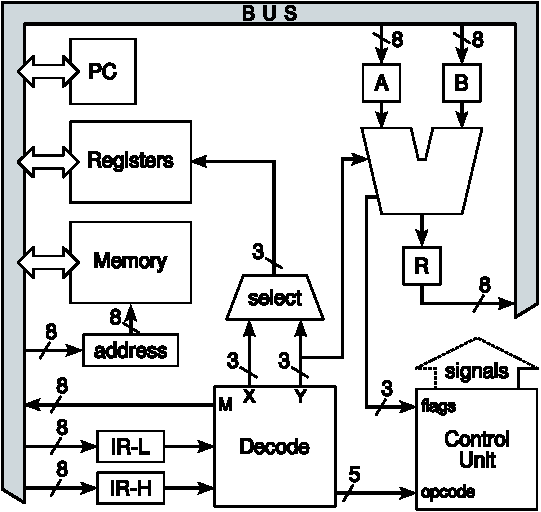
\includegraphics[scale=0.7]{img/arquitectura_micro.pdf}
&
\vspace{-6cm}
\begin{minipage}{8cm}
\begin{itemize}
  \setlength\itemsep{0em}
 \item Arquitectura \emph{von Neumann}, memoria de datos e instrucciones compartida.
 \item 8 registros de propósito general, \texttt{R0} a \texttt{R7}.
 \item 1 registro de propósito específico PC.
 \item Tamaño de palabra de 8 bits e instrucciones de 16 bits.
 \item Memoria de 256 palabras de 8 bits.
 \item Bus de 8 bits.
 \item Diseño microprogramado.
\end{itemize}
\end{minipage}
\\
\end{tabular}
\end{center}

\subsection*{Instrucciones}

Las instrucciones están codificadas en 16 bits.
Los primeros 5 bits indentifican el \texttt{opcode} de la instrucción, el resto de los bits indican los parámetros.
Existen 4 posibles codificaciones de parámetros.

\begin{center}
\begin{tabular}{c|l|l}
Caso & Codificación               & Parámetros \\
\hline
A    & \texttt{OOOOO XXXYYY-----} & \texttt{XXX} = Registro X, \texttt{XXX} = Registro Y o inmediato \\
B    & \texttt{OOOOO XXX--------} & \texttt{XXX} = Registro X\\
C    & \texttt{OOOOO ---MMMMMMMM} & \texttt{MMMMMMMM} = Dirección de memoria o Inmediato\\
D    & \texttt{OOOOO XXXMMMMMMMM} & \texttt{XXX} = Registro X, \texttt{MMMMMMMM} = Dir. de memoria o Imm.\\
\end{tabular}
\end{center}

\noindent Considerando:

\small
\begin{itemize}
  \setlength\itemsep{0em}
 \item \texttt{Rx} o \texttt{Ry}: Indices de registros, número entre \texttt{0} y \texttt{7}.
 \item \texttt{M}: Dirección de memoria o valor inmediato, número de 8 bits.
 \item \texttt{t}: Valor inmediato de desplazamiento, número entre \texttt{0} y \texttt{7}. Se codifica como \texttt{YYY}.
 \item En la columna de codificación, los bits indicados con \texttt{-} son reservados y deben valer cero.
 \item Las instrucciones de \texttt{opcode}: 9, 10, 11, 12, 13, 14, 15, 28, 29 y 30 son instrucciones reservadas.
\end{itemize}
\normalsize

\noindent Las instrucciones soportadas por la arquitectura son las siguientes:

\begin{center}
\begin{tabular}{l|l|l}
Instrucción            & Acción                                                             & Codificación               \\
\hline
\texttt{ADD  Rx, Ry}   & \texttt{Rx} $\leftarrow$ \texttt{Rx + Ry}                          & \texttt{00001 XXXYYY-----} \\  %01
\texttt{ADC  Rx, Ry}   & \texttt{Rx} $\leftarrow$ \texttt{Rx + Ry + flag\_C}                & \texttt{00010 XXXYYY-----} \\  %02
\texttt{SUB  Rx, Ry}   & \texttt{Rx} $\leftarrow$ \texttt{Rx - Ry}                          & \texttt{00011 XXXYYY-----} \\  %03
\texttt{AND  Rx, Ry}   & \texttt{Rx} $\leftarrow$ \texttt{Rx and Ry}                        & \texttt{00100 XXXYYY-----} \\  %04
\texttt{OR   Rx, Ry}   & \texttt{Rx} $\leftarrow$ \texttt{Rx or Ry}                         & \texttt{00101 XXXYYY-----} \\  %05
\texttt{XOR  Rx, Ry}   & \texttt{Rx} $\leftarrow$ \texttt{Rx xor Ry}                        & \texttt{00110 XXXYYY-----} \\  %06
\texttt{CMP  Rx, Ry}   & Modifica \emph{flags} de \texttt{Rx - Ry}                          & \texttt{00111 XXXYYY-----} \\  %07
\texttt{MOV  Rx, Ry}   & \texttt{Rx} $\leftarrow$ \texttt{Ry}                               & \texttt{01000 XXXYYY-----} \\  %08
\hline
\texttt{STR  [M], Rx}  & \texttt{Mem[M]} $\leftarrow$ \texttt{Rx}                           & \texttt{10000 XXXMMMMMMMM} \\  %16
\texttt{LOAD Rx, [M]}  & \texttt{Rx} $\leftarrow$ \texttt{Mem[M]}                           & \texttt{10001 XXXMMMMMMMM} \\  %17
\texttt{STR  [Rx], Ry} & \texttt{Mem[Rx]} $\leftarrow$ \texttt{Ry}                          & \texttt{10010 XXXYYY-----} \\  %18
\texttt{LOAD Rx, [Ry]} & \texttt{Rx} $\leftarrow$ \texttt{Mem[Ry]}                          & \texttt{10011 XXXYYY-----} \\  %19
\hline
\texttt{JMP M}         & \texttt{PC} $\leftarrow$ \texttt{M}                                & \texttt{10100 ---MMMMMMMM} \\  %20
\texttt{JC M}          & Si \texttt{flag\_C=1} entonces \texttt{PC} $\leftarrow$ \texttt{M} & \texttt{10101 ---MMMMMMMM} \\  %21
\texttt{JZ M}          & Si \texttt{flag\_Z=1} entonces \texttt{PC} $\leftarrow$ \texttt{M} & \texttt{10110 ---MMMMMMMM} \\  %22
\texttt{JN M}          & Si \texttt{flag\_N=1} entonces \texttt{PC} $\leftarrow$ \texttt{M} & \texttt{10111 ---MMMMMMMM} \\  %23
\hline
\texttt{INC Rx}        & \texttt{Rx} $\leftarrow$ \texttt{Rx + 1}                           & \texttt{11000 XXX--------} \\  %24
\texttt{DEC Rx}        & \texttt{Rx} $\leftarrow$ \texttt{Rx - 1}                           & \texttt{11001 XXX--------} \\  %25
\texttt{SHR Rx, t}     & \texttt{Rx} $\leftarrow$ \texttt{Rx} \verb|<<| \texttt{t}          & \texttt{11010 XXXYYY-----} \\  %26
\texttt{SHL Rx, t}     & \texttt{Rx} $\leftarrow$ \texttt{Rx} \verb|>>| \texttt{t}          & \texttt{11011 XXXYYY-----} \\  %27
\hline
\texttt{SET Rx, M}     & \texttt{Rx} $\leftarrow$ \texttt{M}                                & \texttt{11111 XXXMMMMMMMM} \\  %31
\end{tabular}
\end{center}

\subsection*{Componentes}

La arquitectura está compuesta por 6 componentes interconectados.
El circuito identificado como \texttt{microOrgaSmall} los integra en un \texttt{dataPath} sobre el lado izquierdo del mismo.
El lado derecho presenta la visualización del estado de los registros.

Los componentes de la arquitectura son: 
\texttt{Registers} (Banco de Registros),
\texttt{PC} (Contador de Programa),
\texttt{ALU} (Unidad Aritmético Lógica),
\texttt{Memory} (Memoria),
\texttt{Decode} (Decodificador de Instrucciones) y
\texttt{ControlUnit} (Unidad de Control)

Cada uno de estos componentes es controlado por medio del conjunto de entradas y salidas descriptas a continuación:

\small

\begin{center}
\begin{tabular}{p{6.4cm}|p{8.2cm}}
\texttt{Registers} (Banco de Registros)              &  \\%Almacena los registros \texttt{R0} a \texttt{R7}.\\
\hline
\texttt{inData(8)} y \texttt{outData(8)}             & Entrada y salida de datos.\\
\texttt{RB\_enIn(1)} y \texttt{RB\_enOut(1)}         & Habilita entrada y salida.\\
\texttt{RB\_inSelect(1)} y \texttt{RB\_outSelect(1)} & Selecciona el índice de \texttt{X} e \texttt{Y}\\
% \hline
\end{tabular}
\end{center}

\begin{center}
\begin{tabular}{p{6.4cm}|p{8.2cm}}
\texttt{PC} (Contador de Programa)          &  \\%Registro PC con señal para incrementar en uno. \\
\hline                                      
\texttt{inValue(8)} y \texttt{outValue(8)}  & Entrada y salida del PC.\\
\texttt{PC\_load(1)}                        & Carga un nuevo valor en el registro.\\
\texttt{PC\_inc(1)}                         & Incrementa el calor actual.\\
\texttt{PC\_enOut(1)}                       & Habilita la salida del valor.\\
% \hline
\end{tabular}
\end{center}

\begin{center}
\begin{tabular}{p{6.4cm}|p{8.2cm}}
\texttt{ALU} (Unidad Aritmético Lógica) &  \\%Componente para operaciones artiméticas y lógicas, con registros de entrada, salida y flags.\\
\hline
\texttt{A(8)}, \texttt{B(8)}, \texttt{out(8)} y \texttt{flags(3)}   & Entradas y salidas de la ALU.\\
\texttt{ALU\_enA(1)}, \texttt{ALU\_enB(1)} y \texttt{ALU\_enOut(1)} & Habilitación de entradas y salidas. \\
\texttt{ALU\_opW(1)}                                                & Indica si se deben escribir los \emph{flags}.\\
\texttt{ALU\_OP(4)}                                                 & Indica la operación a realizar por la ALU.\\
% \hline
\end{tabular}
\end{center}

\begin{center}
\begin{tabular}{p{6.4cm}|p{8.2cm}}
\texttt{Memory} (Memoria)                   &  \\%Memoria de lectura y escritura, almacena datos de 8 bits con direcciones de 8 bits.\\
\hline                                      
\texttt{inData(8)} y \texttt{outData(8)}    & Entrada y salida de datos.\\
\texttt{MM\_addr}                           & Dirección de memoria donde leer.\\
\texttt{MM\_enOut}                          & Habilitación de la salida.\\
\texttt{MM\_load}                           & Indica si leer o escribir. \\
\texttt{MM\_enAddr}                         & Habilita cargar la dirección. \\
% \hline
\end{tabular}
\end{center}

\begin{center}
\begin{tabular}{p{6.4cm}|p{8.2cm}}
\texttt{Decode} (Decodificador de Inst.)    &  \\%Decodifica una instrucción, identifica su opcode, les registros y parámetros.\\
\hline
\texttt{halfInst(8)}                        & Entrada de datos (media instrucción)\\
\texttt{DE\_loadL(8)} y \texttt{DE\_loadH(8)} & Indica cargar la mitad alta o baja.\\
\texttt{opcode(5)}                          & Salida de Opcode decodificado.\\
\texttt{indexX(3)} y \texttt{indexY(3)}     & Salidas de índices de registros.\\
\texttt{valueM(8)}                          & Salida de valor inmediato o dirección.\\
% \hline
\end{tabular}
\end{center}

\begin{center}
\begin{tabular}{p{6.4cm}|p{8.2cm}}
\texttt{ControlUnit} (Unidad de Control) &  \\%Secuenciador de microinstrucciones, genera señales que ejecutan el ciclo de instrucción.\\
\hline
\texttt{inOpcode(5)}                                                 & Entrada de \emph{Opcode}.\\
\texttt{flags(3)}                                                    & Entrada de \emph{flags}.\\
\texttt{RB\_enIn(1)} y \texttt{RB\_enOut(1)}                         & Señales de habilitación para Registros\\
\texttt{RB\_inSelect(1)} y \texttt{RB\_outSelect(1)}                 & Señales de selección para Registros\\
\texttt{MM\_enOut(1)} y \texttt{MM\_load(1)}                         & Señales para la Memoria.\\
\texttt{MM\_enAddr(1)}                                               & Habilita cargar la dirección.\\
\texttt{ALU\_enA(1)}, \texttt{ALU\_enB(1)} y \texttt{ALU\_enOut(1)}  & Señales de habilitación de la ALU.\\
\texttt{ALU\_opW(1)}, \texttt{ALU\_OP(4)}                            & Señales de control de la ALU.\\
\texttt{PC\_load(1)}, \texttt{PC\_inc(1)} y \texttt{PC\_enOut(1)}    & Señales de control de PC.\\
\texttt{DE\_enOutImm(1)}                                             & Habilita la entrada al bus de un valor inmediato.\\
\texttt{DE\_loadL(8)} y \texttt{DE\_loadH(8)}                        & Indica cargar la mitad alta o baja.\\
% \hline
\end{tabular}
\end{center}

Algunas de estas entradas y salidas están conectadas directamente al bus del sistema, mientras que otras son utilizadas como señales de control.
Estas últimas están directamente conectadas a la unidad de control (\texttt{UC}).

\subsection*{Micro-Instrucciones}

Las micro-instrucciones corresponden a la secuencia de señales necesarias para resolver una instrucción.
En este diseño, tanto la operación de \emph{fetch} como \emph{decode} son ejecutadas por medio de micro-instrucciones.
Una vez identificada la instrucción a ejecutar, la operación de \emph{execute} también es realizada por código de micro-instrucciones.

Las micro-instrucciones son almacenadas en una memoria destinada para tal fin, que forma parte del componente \texttt{UC}.
Está memoria contiene palabras de 32 bits y direcciones de 9 bits.
Cada uno de los 32 bits de la palabra corresponde a una señal para algún componente según se detalla más adelante.
Estas señales pueden estar directamente conectadas a un componente o ser señales internas de la \texttt{UC}.

La \texttt{UC} funciona como un secuenciador de señales.
El registro \texttt{microPC} dentro de la \texttt{UC} opera como un contador de programa, que indica la dirección de la próxima micro-instrucción a ejecutar.
Toma como entradas el \emph{opcode} de la instrucción a ejecutar y los valores de \emph{flags} desde la \texttt{ALU}.

Inicialmente \texttt{microPC} vale cero, donde las señales generadas correspondientes a la etapa de \emph{fetch}.
En esta se carga desde la memoria la próxima instrucción a ser ejecutada indicada por el \texttt{PC}.
Como la memoria direcciona a byte, y las instrucciones ocupan dos bytes, el proceso de \emph{fetch} debe cargar dos valores desde memoria.
Estos valores son enviados a la unidad de decodificación (\emph{DE}).
Esta última genera cuatro salidas \texttt{M}, \texttt{X}, \texttt{Y} y \texttt{OP}.
Las primeras tres corresponden a los parámentros de la instrucción y la restante a su \emph{opcode}.
Luego la \texttt{UC} carga en el \texttt{microPC} el valor \emph{opcode} \verb|<<| \texttt{4}, es decir, agrega cuatro ceros en los bits menos significativos del \emph{opcode}.
Las siguientes micro-instrucciones corresponden a la secuencia de señales para resolver la instrucción indicada por el \emph{opcode}.
Una vez resuelta la instrucción, el ciclo comienza nuevamente seteando \texttt{microPC} en cero.

\bigskip

\noindent La estructura de la memoria de micro-instrucciones es la siguiente:

\small
\begin{center}
\begin{tabular}[t]{l|lcl|lcl|lcl|l}
Dirección          & Inst.         & & Dirección          & Inst.         & & Dirección          & Inst.         & & Dirección          & Inst.         \\  
\cline{1-2} \cline{4-5} \cline{7-8} \cline{10-11}
\texttt{00000xxxx} & \texttt{fetch}& & \texttt{01000xxxx} & \texttt{MOV}  & & \texttt{10000xxxx} & \texttt{STR}  & & \texttt{11000xxxx} & \texttt{INC}  \\
\texttt{00001xxxx} & \texttt{ADD}  & & \texttt{01001xxxx} & \texttt{-}    & & \texttt{10001xxxx} & \texttt{LOAD} & & \texttt{11001xxxx} & \texttt{DEC}  \\
\texttt{00010xxxx} & \texttt{ADC}  & & \texttt{01010xxxx} & \texttt{-}    & & \texttt{10010xxxx} & \texttt{STR*} & & \texttt{11010xxxx} & \texttt{SHR}  \\
\texttt{00011xxxx} & \texttt{SUB}  & & \texttt{01011xxxx} & \texttt{-}    & & \texttt{10011xxxx} & \texttt{LOAD*}& & \texttt{11011xxxx} & \texttt{SHL}  \\
\texttt{00100xxxx} & \texttt{AND}  & & \texttt{01100xxxx} & \texttt{-}    & & \texttt{10100xxxx} & \texttt{JMP}  & & \texttt{11100xxxx} & \texttt{-}    \\
\texttt{00101xxxx} & \texttt{OR}   & & \texttt{01101xxxx} & \texttt{-}    & & \texttt{10101xxxx} & \texttt{JC}   & & \texttt{11101xxxx} & \texttt{-}    \\
\texttt{00110xxxx} & \texttt{XOR}  & & \texttt{01110xxxx} & \texttt{-}    & & \texttt{10110xxxx} & \texttt{JZ}   & & \texttt{11110xxxx} & \texttt{-}    \\
\texttt{00111xxxx} & \texttt{CMP}  & & \texttt{01111xxxx} & \texttt{-}    & & \texttt{10111xxxx} & \texttt{JN}   & & \texttt{11111xxxx} & \texttt{SET}  \\
\end{tabular}
\end{center}
(\texttt{*}) Instrucciones con direccionamiento indirecto a memoria.
\normalsize

\bigskip

Los datos almacenados en la memoria de micro-instrucciones corresponden a señales para los distintos componentes del sistema.
La siguiente tabla indica a qué bit de micro-instrucción corresponde cada señal.

\small
\begin{center}
\begin{tabular}[t]{llllllll}
\texttt{\fbox{00}} & \texttt{RB\_enIn}           & \texttt{\fbox{08}} & \texttt{ALU\_enA}   & \texttt{\fbox{16}} & \texttt{JC\_microOp} & \texttt{\fbox{24}} & \texttt{DE\_enOutImm}   \\
\texttt{\fbox{01}} & \texttt{RB\_enOut}          & \texttt{\fbox{09}} & \texttt{ALU\_enB}   & \texttt{\fbox{17}} & \texttt{JZ\_microOp} & \texttt{\fbox{25}} & \texttt{DE\_loadL}      \\
\texttt{\fbox{02}} & \texttt{RB\_selectIndexIn}  & \texttt{\fbox{10}} & \texttt{ALU\_enOut} & \texttt{\fbox{18}} & \texttt{JN\_microOp} & \texttt{\fbox{26}} & \texttt{DE\_loadH}      \\
\texttt{\fbox{03}} & \texttt{RB\_selectIndexOut} & \texttt{\fbox{11}} & \texttt{ALU\_opW}   & \texttt{\fbox{19}} & \texttt{-}           & \texttt{\fbox{27}} & \texttt{-}              \\
\texttt{\fbox{04}} & \texttt{MM\_enOut}          & \texttt{\fbox{12}} & \texttt{ALU\_OP}    & \texttt{\fbox{20}} & \texttt{PC\_load}    & \texttt{\fbox{28}} & \texttt{-}              \\
\texttt{\fbox{05}} & \texttt{MM\_load}           & \texttt{\fbox{13}} & \texttt{ALU\_OP}    & \texttt{\fbox{21}} & \texttt{PC\_inc}     & \texttt{\fbox{29}} & \texttt{-}              \\
\texttt{\fbox{06}} & \texttt{MM\_enAddr}         & \texttt{\fbox{14}} & \texttt{ALU\_OP}    & \texttt{\fbox{22}} & \texttt{PC\_enOut}   & \texttt{\fbox{30}} & \texttt{load\_microOp}  \\
\texttt{\fbox{07}} & \texttt{-}                  & \texttt{\fbox{15}} & \texttt{ALU\_OP}    & \texttt{\fbox{23}} & \texttt{-}           & \texttt{\fbox{31}} & \texttt{reset\_microOp} \\
\end{tabular}
\end{center}
\normalsize

\bigskip

La codificación de las operaciones de la unidad artimético lógica es la siguiente:

\small
\begin{center}
\begin{tabular}[t]{c|lcc|lcc|lcc|l}
Código        & Operación    & & Código        & Operación    & & Código        & Operación    & & Código        & Operación        \\
\cline{1-2}                      \cline{4-5}                       \cline{7-8}                     \cline{10-11}
\texttt{0000} & \texttt{Reservada}   & & \texttt{0100} & \texttt{AND} & & \texttt{1000} & \texttt{SHR} & & \texttt{1100} & \texttt{cte0x00} \\
\texttt{0001} & \texttt{ADD} & & \texttt{0101} & \texttt{OR}  & & \texttt{1001} & \texttt{SHL} & & \texttt{1101} & \texttt{cte0x01} \\
\texttt{0010} & \texttt{ADC} & & \texttt{0110} & \texttt{XOR} & & \texttt{1010} & \texttt{-}   & & \texttt{1110} & \texttt{cte0x02} \\
\texttt{0011} & \texttt{SUB} & & \texttt{0111} & \texttt{CMP} & & \texttt{1011} & \texttt{-}   & & \texttt{1111} & \texttt{cte0xFF} \\
\end{tabular}
\end{center}
\normalsize

\section*{Herramientas}

Se cuenta con dos herramientas: un programa ensamblador, que transforma código ASM en código binario, y un generador de micro-instrucciones.
Este último genera a partir de un archivo de descripción de señales el código binario de micro-instrucciones.

\begin{center}
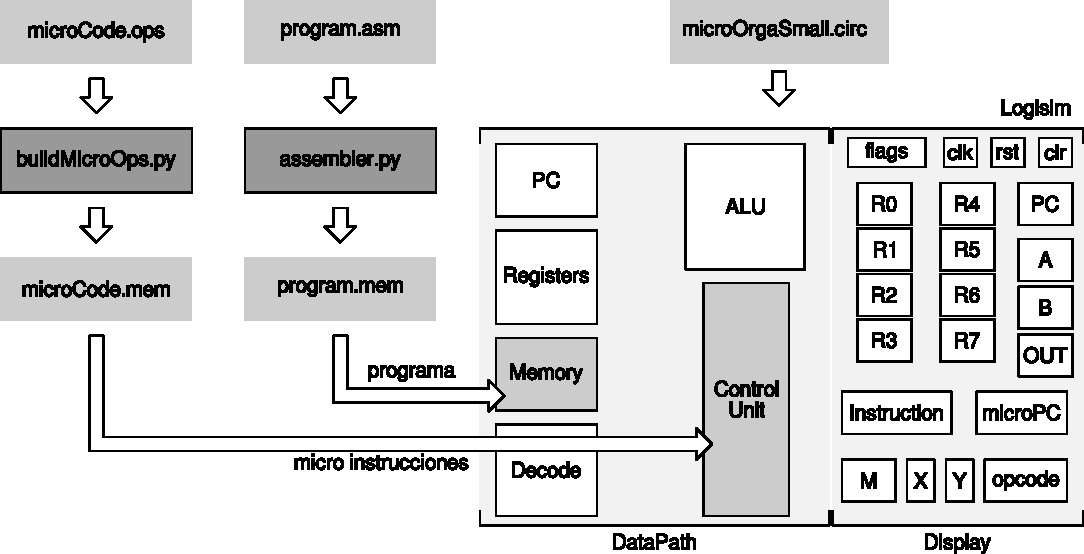
\includegraphics[scale=0.6]{img/herramientas.pdf}
\end{center}


\subsection*{Ensamblador (\texttt{assembler.py})}

El ensamblador toma como entrada un archivo de texto con la lista de mnemónicos de instrucciones y genera el código binario del programa.
Las instrucciones soportadas son todas las descriptas por la arquitectura, además el ensamblador soporta el uso de etiquetas y comentarios.
Las etiquetas pueden ser cualquier cadena de caracteres finalizada en ``:''. Una vez declarada, puede ser utilizada en cualquier parte del código, incluso como parámetro o valor inmediato.
Para declarar un comentario, se utiliza el caracter ``;''.
Todo el texto luego de la primera aparición de este será considerado comentario.
El ensamblador además soporta declarar valores inmediatos.
Para esto se utiliza la palabra reservada \texttt{DB} y luego de esta un valor númerico inmediato.
Este será incluido directamente en el código generado.

\subsection*{Generador de Micro-instrucciones (\texttt{buildMicroOps.py})}

El generador de micro-instrucciones toma como entrada un archivo de descripción de señales que respeta la siguiente sintaxis:

\small
\begin{verbatim}
<binary_opcode>:
<signal_1> <signal_2> <signal_n>
...
<signal_1> <signal_2> <signal_n>
\end{verbatim}
\normalsize

\noindent donde \verb|<binary_opcode>| corresponde al valor de \emph{opcode} a codificar en binario y \verb|<signal>| a un nombre de señal.
Las señales pueden ser indicadas por el nombre de la misma o como: \verb|<signal>=<x>| donde \verb|x| indica el valor de la señal.
Para señales de más de un bit, como \verb|ALU_OP| se debe utilizar el número entero decimal correspondiente.
En particular, para la señal mencionada, se puede utilizar directamente el nombre de la operación en la \texttt{ALU}.
Si no se indica el valor que debe tomar la señal, se utiliza 1.

\noindent Por ejemplo, para la codificación de la instruccón \verb|ADD|:

\small
\begin{verbatim}
00001: ; ADD
    RB_enOut  ALU_enA  RB_selectIndexOut=0   ; ALU_A := Rx
    RB_enOut  ALU_enB  RB_selectIndexOut=1   ; ALU_B := Ry
    ALU_OP=ADD ALU_opW                       ; ALU_ADD
    RB_enIn   ALU_enOut RB_selectIndexIn=0   ; Rx := ALU_OUT
    reset_microOp
\end{verbatim}
\normalsize

\noindent Notar que la señal \verb|ALU_OP| es completada con un texto que indica la operación de la ALU a realizar.

\subsection*{Uso}

Una vez dentro de \emph{Logisim} se debe cargar el circuito de \texttt{OrgaSmall}.
Para cargar un programa, se debe entrar en el circuito \texttt{memory} y una vez seleccionada la memoria, utilizar el comando \emph{load} para cargar un nuevo programa.
Para modificar el código de micro-instrucciones, se debe entrar al circuito \texttt{controlUnit} y con el mismo procedimiento anterior, cargar el nuevo código de micro-instrucciones.
Recordar que el \texttt{PC} comienza siempre en cero, y esta es la primera instrucción a ejecutar.

\vspace{1cm}

% \newpage
\section*{Implementación en \emph{Logisim}}

\vspace{0.5cm}

\begin{center}
 \begin{tabular}[t]{c}
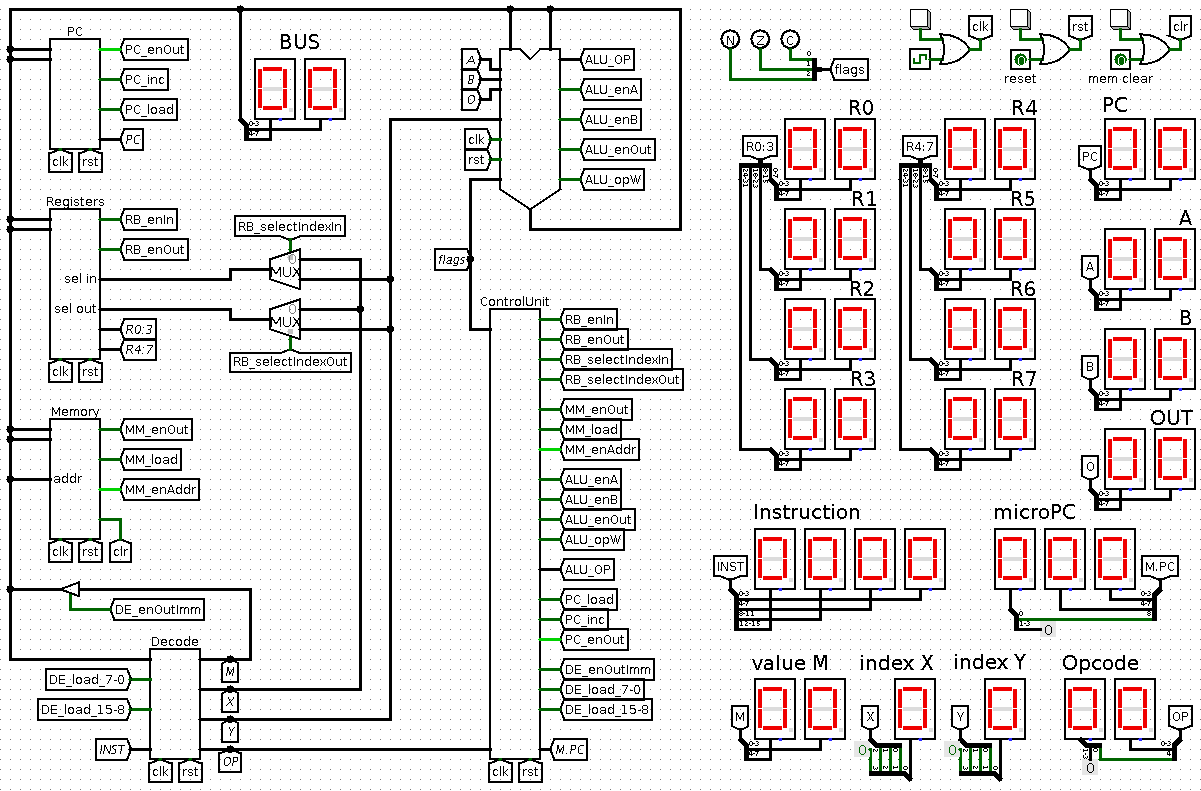
\includegraphics[scale=0.3]{img/0_dataPath.png} \\
\hline
Data Path \\ \hline
\end{tabular}
\end{center}

\vspace{0.5cm}

\begin{center}
\begin{tabular}[t]{c}
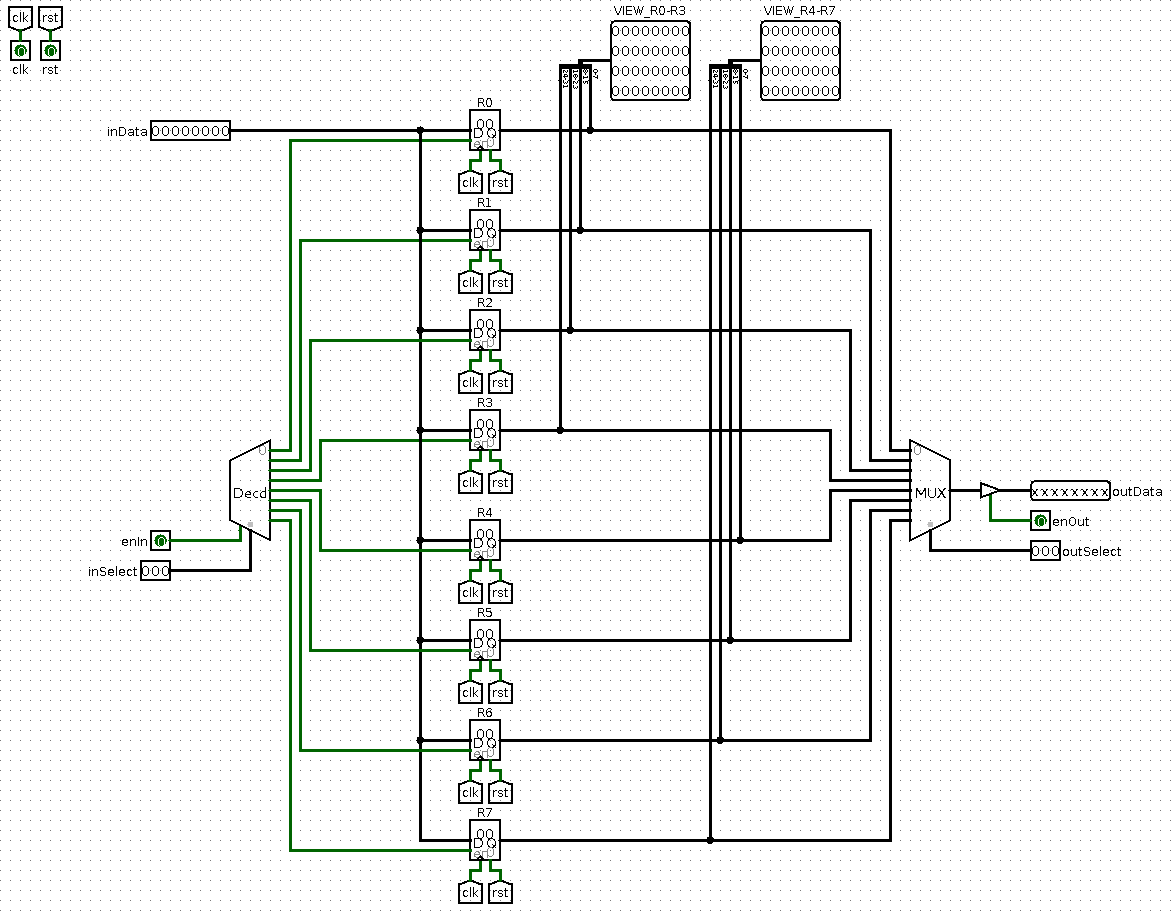
\includegraphics[scale=0.3]{img/1_registers.png} \\
\hline
Registros\\ \hline
\end{tabular}
\end{center}

\vspace{0.5cm}

\begin{center}
 \begin{tabular}[t]{c}
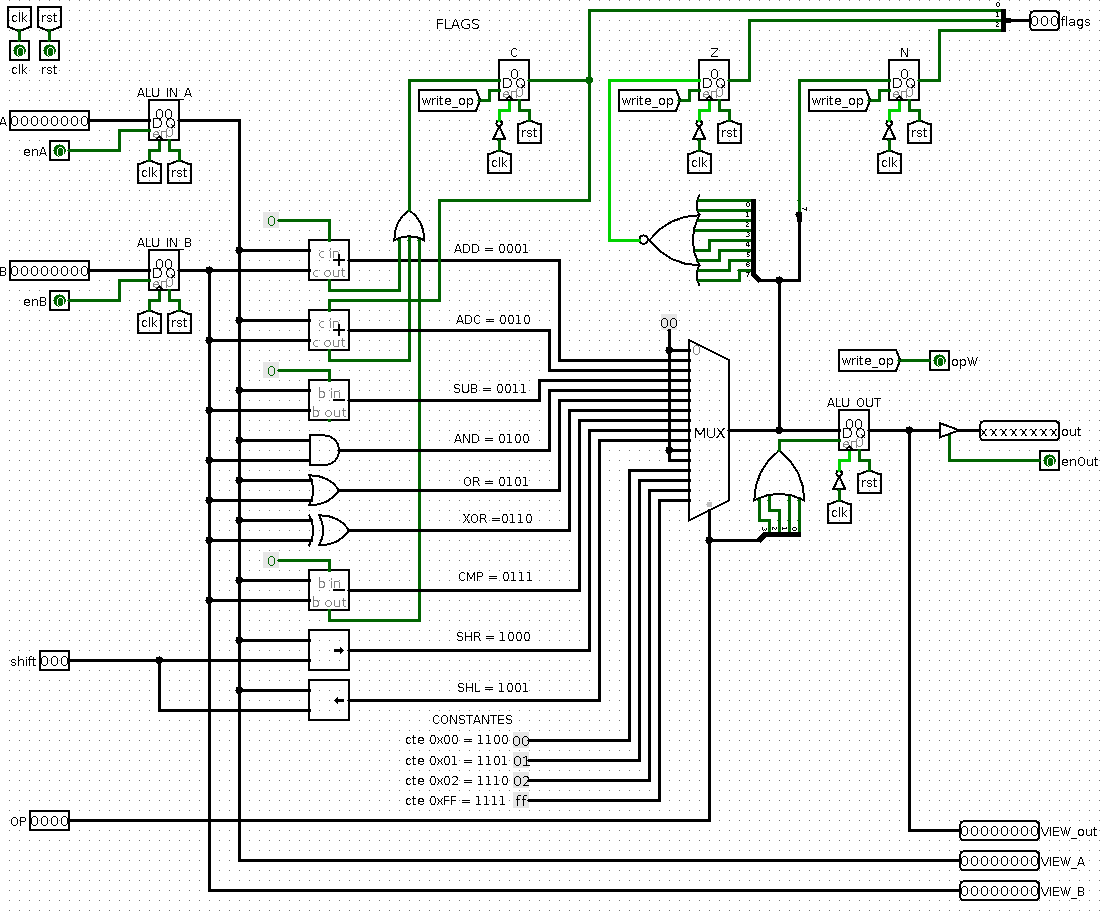
\includegraphics[scale=0.3]{img/4_ALU.png} \\
\hline
Unidad Aritmético Lógica\\ \hline
\end{tabular}
\end{center}

\vspace{0.5cm}

\begin{center}
\begin{tabular}[t]{c|c}
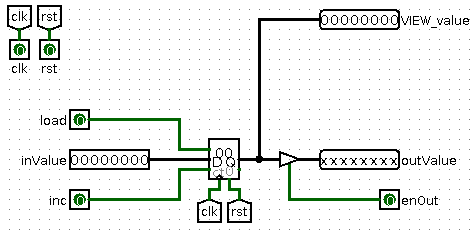
\includegraphics[scale=0.3]{img/2_PC.png} & 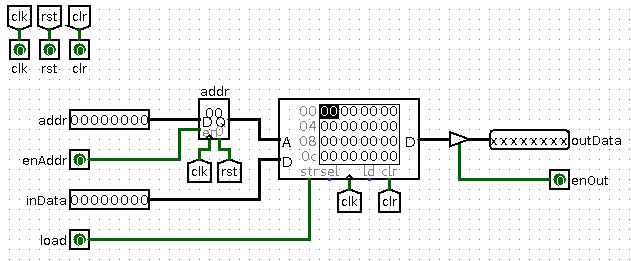
\includegraphics[scale=0.3]{img/5_Memory.png}\\
\hline
Contador de programa & Memoria de Instrucciones\\ \hline
\end{tabular}
\end{center}

\vspace{0.5cm}

\begin{center}
\begin{tabular}[t]{c}
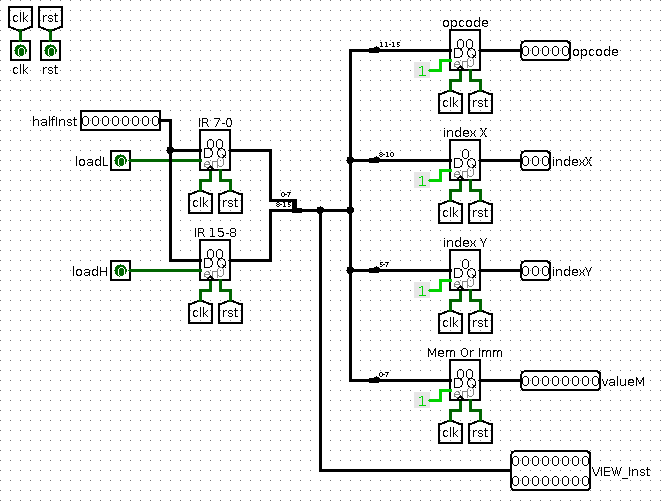
\includegraphics[scale=0.3]{img/6_Decode.png}\\
\hline
Decodificador\\ \hline
\end{tabular}
\end{center}

\vspace{0.5cm}

\begin{center}
\begin{tabular}[t]{c}
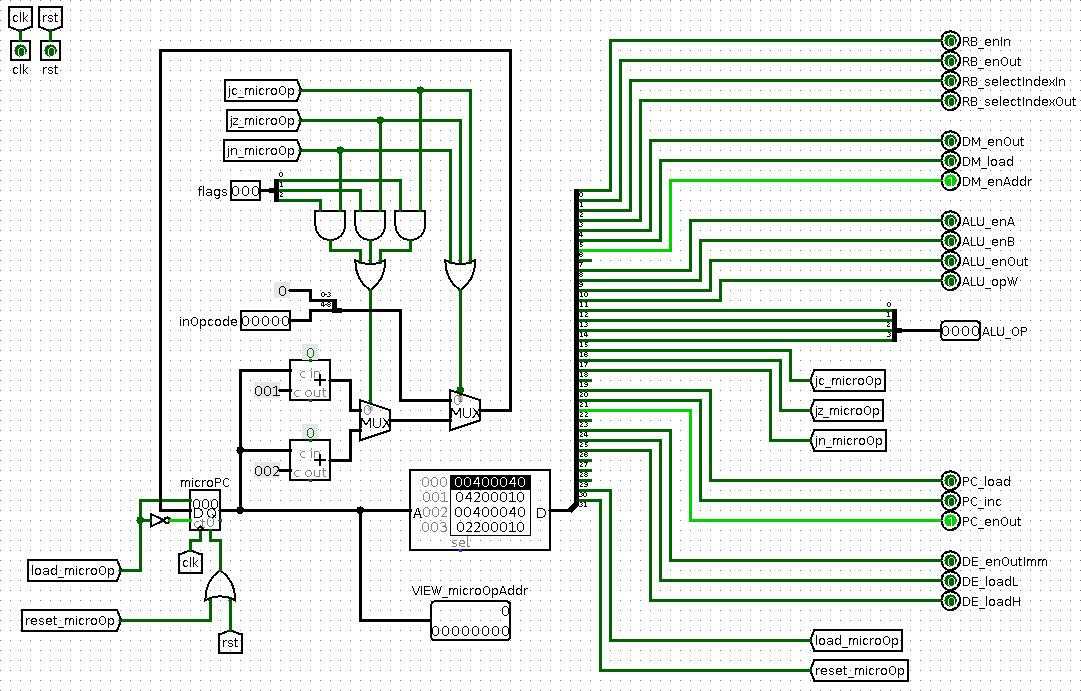
\includegraphics[scale=0.3]{img/7_ControlUnit.png}\\
\hline
Unidad de Control\\ \hline
\end{tabular}
\end{center}

\end{document}
